\documentclass{acm_proc_article-sp}
\usepackage[lined,boxed,commentsnumbered]{algorithm2e}
\usepackage{amsmath}
\usepackage{graphicx}
\usepackage{url}
\usepackage{multirow}

\begin{document}

\title{PushUp: An event-based http Long-polling Server}

\numberofauthors{2}
\author{
% 1st. author
\alignauthor
Kai Liu \\
       \affaddr{Very Large Information System}\\
       \affaddr{Carnegie Mellon University}\\
       \email{hfevers@gmail.com}
% 2nd. author
\alignauthor
Yilun Cui \\
       \affaddr{Very Large Information System}\\
       \affaddr{Carnegie Mellon University}\\
       \email{yiluncui@gmail.com}
}

\maketitle

\begin{abstract} 

The ``long-polling" is a server push technology that makes the delivery the 
latest updates from server to client more ``instant". With long polling, 
when a client requests updates from the server, the server
will keep the request connection open if there is no available update yet. 
The server sends the complete response to the client only when the interested
information becomes available or after a suitable timeout.

However this solution may require the server to hold large number of open 
connections for in the server side. To efficiently manage these connections
and reduce the complexity of web development, we proposed an event-driven, 
dedicated long-polling server to provide efficient and scalable long polling
services for the underlying web servers. To prove its efficiency, we compare
the performance of PushUp server and several other server-side event 
notification methods. The experimental results confirms the PushUp server's 
excellent capacity in serving large number of concurrent connections with 
much less resource.

\end{abstract}
\section {Introduction}
In computer science the term ``Push" (also known as ``server push''), describes a type of Internet-based communication where the request for a given transaction is initiated by the server. By contrast the term ``pull" describes the client-initiated communication\cite{PushOverview}.

Traditionally, the http web server is the role model of the pull model, where the clients initiate the request and the server respond it. However, with the increasing popularity of Ajax\cite{Ajax} people are no longer satisfy with the old-fashion request-response communication. Instead, they are looking for more ''interactive" websites. That is, the client should be informed of the latest updates from the server as soon as possible.  

Unfortunately, the classical http communication model, for security reasons, imposes a limitation that all browser/server communication to be initiated by the browser. So in order to build the ``interactive" web page, people resort to many different approaches.

\begin{itemize}
\item Client polling: one approach is to let the browser poll the latest message from server periodically. However, this method can result in large amount of HTTP requests.
\item Plugins: since the http itself doesn't provide any original mechanism for server push, many resort to various plugins to achieve more complicated server/client communication. Plugins, such as Flash, Silverlight, Javalet, etc, were used for this purpose. However plugins is non-standard and requires users' extra effort to install and configure them. Also, on the development side, the plugins may lead to the incompatibility issues among different operating systems or browsers. 
\end{itemize}

Given those drawbacks, we focus on the another solution: long polling\cite{LongPolling}.  With long polling the http server will not terminate a connection after the client sends the polling request; instead, the server will keep the connection open for a period of time until (1) a new message arrives in the server side or (2) the request expired. 

This strategy enables the server side to notify the clients immediately if events occurred. However long polling also has its own draw back: keeping a lot of active connections may consume huge amount of server resource. For small scale websites this will not be a problem, but for websites with large traffic, the number of active connections may become a serious bottleneck.

To address these problems, in this project we present the event-based PushUp\cite{UnixBook} system that is dedicated to handle large active connections.

As illustrated in figure [TODO: A PIC IS NEEDED], the PushUp lies in between of clients and backend servers. It has two responsibilities:

\begin {itemize}
\item An event-based reverse proxy\cite{ReverseProxy} retrieves resources on behalf of a client from one or more servers. When there are many requests coming to the server, the server needs to create many parallel threads/processes and keep them running while client will close connection. If client has slow connection, web server process will wait too long and resource consumption will increase very fast.
\item An event-based Message Queue\cite{PubSub} that can keep active connections with very low overhead. The event-based message queue is dedicated for the long polling request from the client. In this architecture the backend servers are the publisher and the clients the subscribers.
\end {itemize}


\section {System Overview\\}

\subsection{Design Goals and Rationales\\}
The design of the PushUp server is driven by the following rationales.
\begin{itemize}
\item {\bf Large Concurrent Connections}:
    As the long polling technologies requires the server to keep the polling
    request active for a period of time, large number of concurrent clients 
    will generate lots of active connections. One of the most goal of PushUp
    is to minimize the cost of maintaining these active concurrent connections,
    which can in turn enhance the system's scalability.
     
    The key to reduce the cost is the event-driven notification mechanism 
    provided by the operating systems. Unlike the multi-process or 
    multithreading concurrent model, the event-driven concurrency model 
    requires much less resource to maintain the connections.

\item {\bf Transparency}: Although event-driven concurrency significantly 
    reduce the maintenance cost, it is impractical to have all the web 
    server to be implemented in event-driven programming style. Thus, the 
    PushUp server provides the dedicated event-driven long polling services
    for all underlying web servers. We hope the introduction of PushUp server
    requires minimal modification on the web servers and hides its existence
    from the clients.

\item {\bf Low Latency}: Adding an intermediate layer in between of the 
    clients and web servers will inevitably create some overhead. 
    The PushUp server should make sure that the extra costs should be within
    an ``acceptable" range.

\item {\bf Scalability}: The PushUp Server is designed to handle large number of
    active connections. We introduces mechanisms to make PushUp more able to
    handle this problem. 

\end{itemize}

\subsection{System Overview\\}

TODO: a figure to illustrate the main idea.

\begin{figure}[htb!]
\centering%
    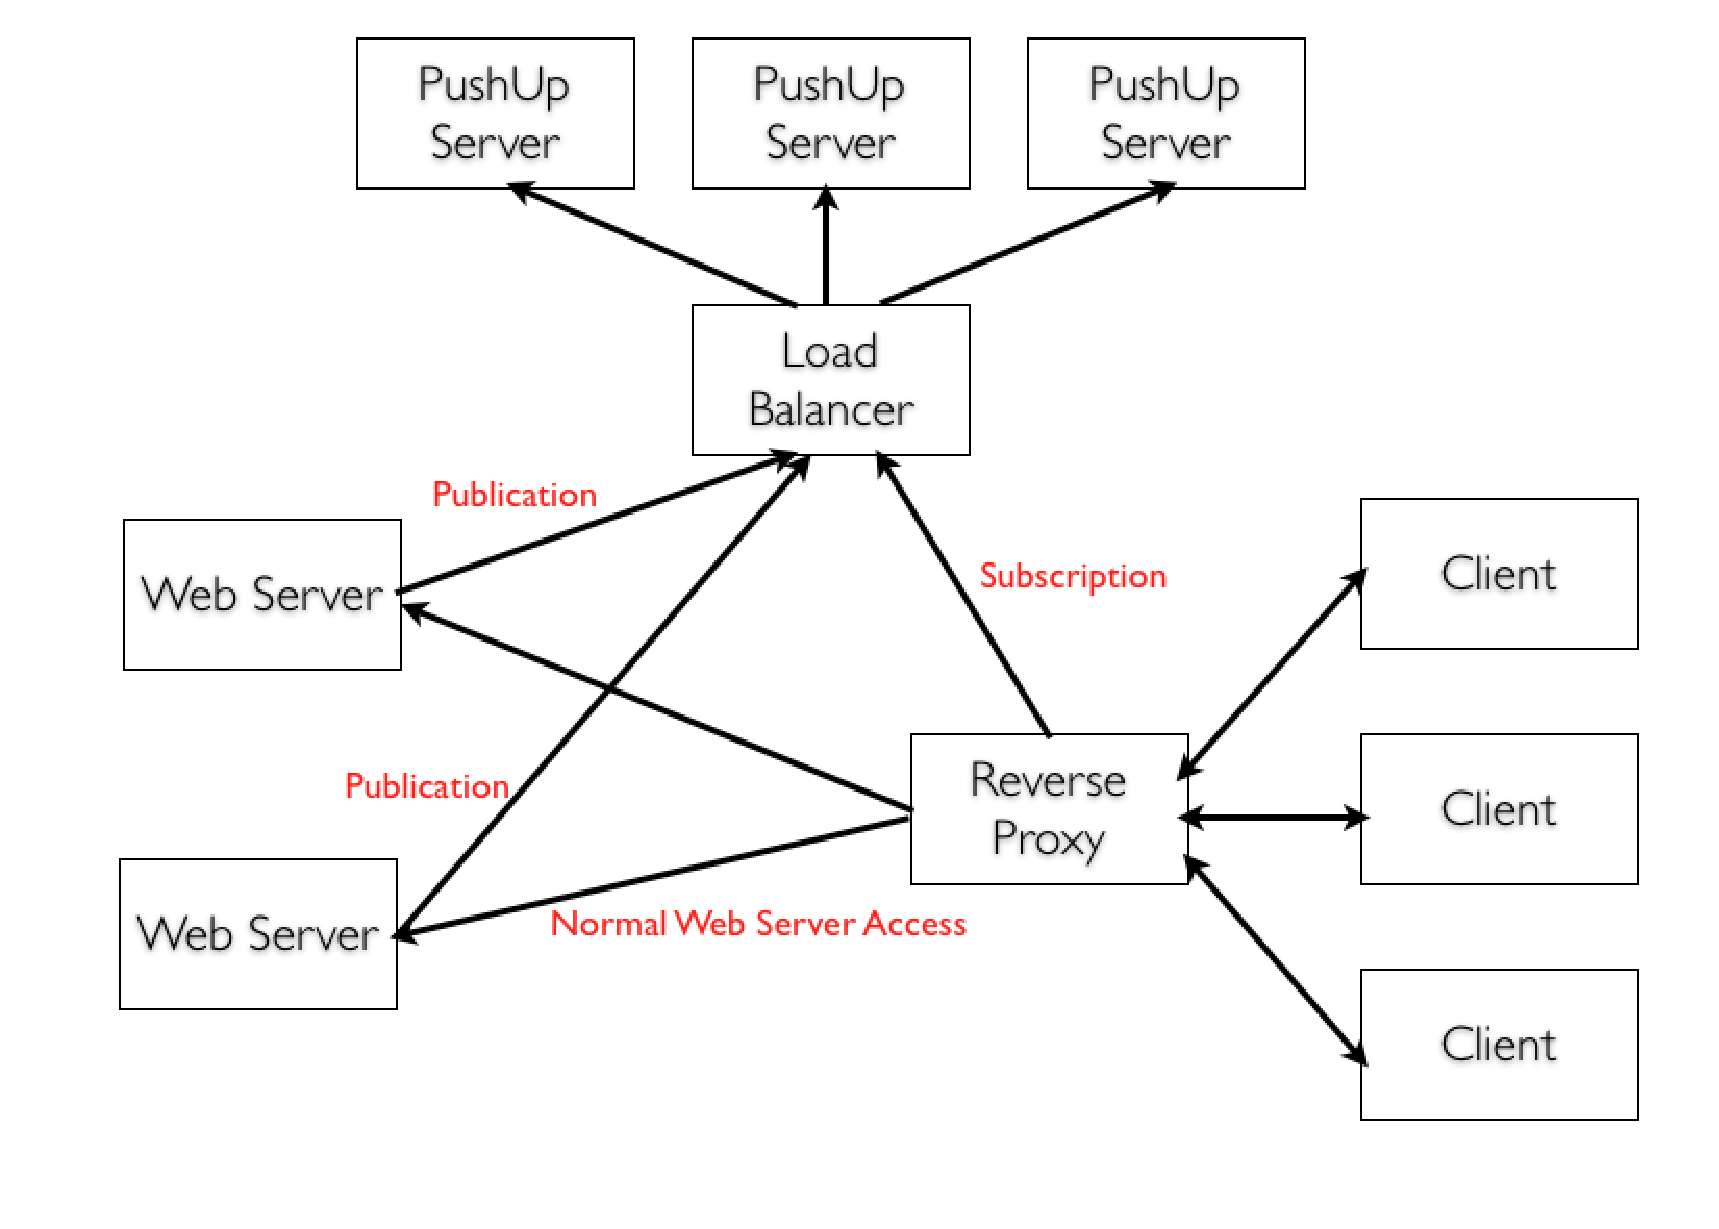
\includegraphics[scale=0.30]{figures/pushup.eps}
    \caption{PushUp Architecture}
    \label{fig:eventloop}
\end{figure}

TODO: Overall description of such design. and how it matches the rationale mentioned above.

TODO: should add add picture with the detailed architecture of the PushUp Server.


\section {Design and Implemenation\\}

\subsection{Reactor Model\\}
The PushUp Server runs atop of the Twisted framework\cite{Twisted}, which is a event-based network programming framework. The highlight of the Twisted is its reactor model\cite{Reactor}.

The reactor is the core of the event loop inside the framework. Event loop is a higher level abstraction of multiplexing model in Linux/Unix (kqueue in Unix and epoll in Linux).

The responsiblities of a event loop is to wait for and dispatches incoming ``events", which will trigger the internal or external "event handlers"(named ``Deferred" in twisted framework, which can be understood as the advanced ``callback" function).

The event loop runs in a single thread and its workflow loop is illustrated in Figure\ref{fig:eventloop}.

\begin{figure}[htb!]
\centering%
    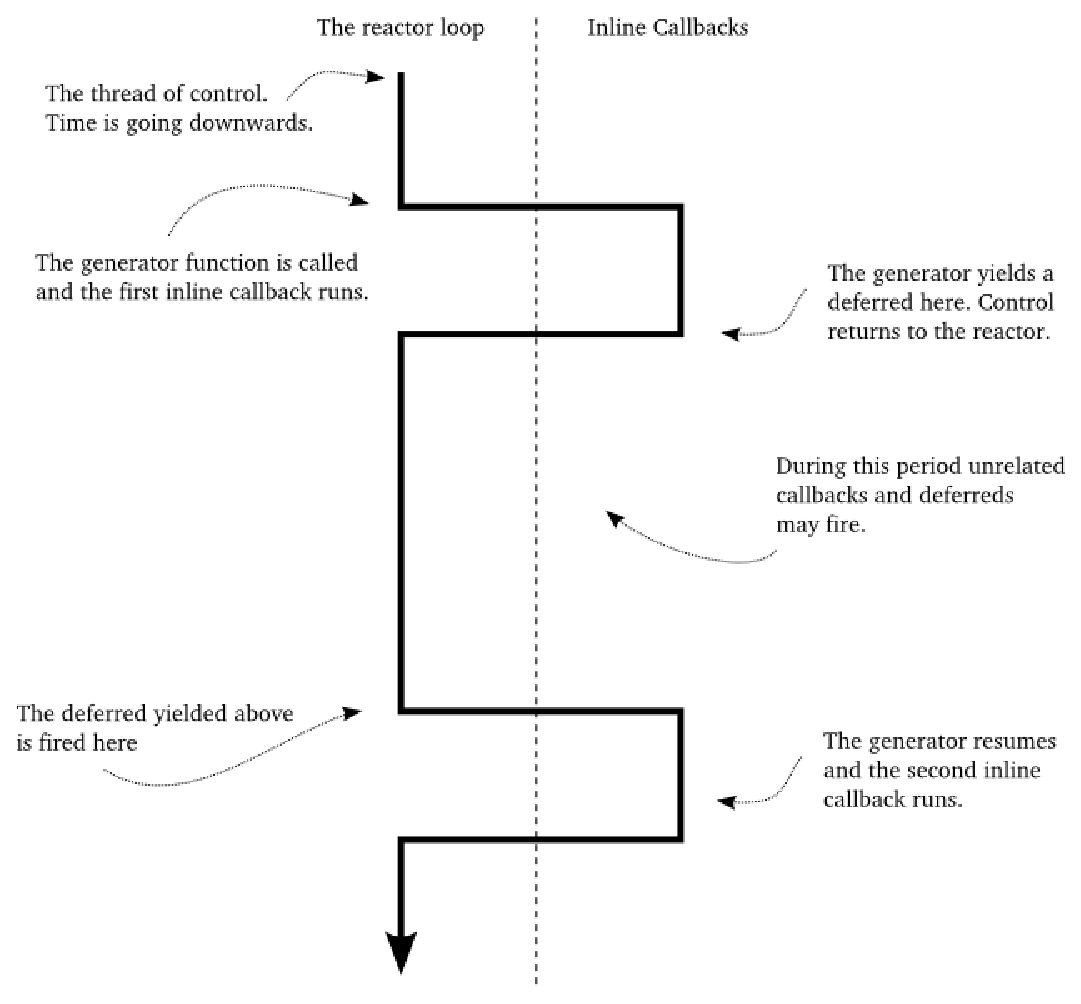
\includegraphics[scale=0.50]{figures/eventloop.eps}
    \caption{Twisted Event Loop}
    \label{fig:eventloop}
\end{figure}


\subsection{Reverse Proxy\\}

How it works, with more details.

\subsection{Message Queue\\}

Pub/Sub: with more details

Publisher: 

    * General design

    * Backend sever connect to the 

Subscriber: 

    * General Design
    * Client Design
    * Just 50 seconds

Message Management

Subscriber

Internal Data structure: what are the highlight of such design.

\subsection{Load Balancer\\}

HAProxy -- based on xxxx.


\section {Evaluation\\}
 
In this section, we conducted experiments to evaluate the performance of 
several web-based event\footnote{the term ``event" here refers to the ``latest 
updates in the server side", which differs from the meaning in ``event-driven"
} notification mechanisms. We also evaluated PushUp servers' performance with
different server numbers.

To better characterize the performance of the PushUp server, we chose ``Client
Pulling" and ``Multithreadeding long polling" as the baseline. The PushUp
adopted the Event-driven long polling mechanism.

\begin{itemize}
    \item {\bf Client Pulling (CP): } In this method the client side initiates 
        an http request to the server to pull the latest updates on a regular 
        basis.
    \item {\bf Multithreadeding long polling(MLP): } This method realizes the 
        long polling by multi threads. For each incoming polling request, the
        server will create a thread waiting for the latest updates.
    \item {\bf Event-driven long polling(ELP): } This method realizes the long
        polling by event-driven mechanism. This method keeps all the polling 
        requests within a single thread.
\end{itemize}

\subsection{Settings \\}

\subsubsection{Evaluation Metrics \\}
In the evaluation, we used the following control variables to control in
the experiments.

\begin{itemize}
    \item {\bf Number of concurrent connections}: This variable allows us 
         to evaluate the scalability of different methods.
    \item {\bf Publish Interval}: This variable controls the frequency of 
         event publication by the server. 
    \item {\bf Polling interval}: This variable determines how long will 
        the method send a polling request to the server. For client 
        pulling, it sends polling request at a regular basis; as for
        long polling methods, they send polling request (1) after they
        just received a new update or (2) after a suitable timeout.
\end{itemize}

And we used the following metrics to evaluate the performance of different
methods.
\begin{itemize}
    \item {\bf Network Traffic (NT)}: NT evaluates the network usage for
        different event notification methods.
    \item {\bf Mean Publish Trip Time (MPT)}: The publish trip-time is 
        the time elapsed between the creation of a data by the server and 
        its reception by the client. It shows how long it takes for the 
        client to be updated when an event occurs.
    \item {\bf Received Message Percentage (RMP)}: RMP indicates the data 
        loss in during the network communication. 
    \item {\bf Server Memory Usage (SMU)}: In many real world long polling 
        system, the polling requests spent most of their time waiting for 
        the new events.[source needed] Thus, memory cost for each idle 
        polling requests is critical to the overall performance.
\end{itemize}

\subsubsection{Evaluation Environment \\}
The experiments are done in CMU's PEACE cluster. Each machine in the cluster 
has a 4 CPU cores(AMD Opteron Processor 4130, 2600 MHz, 512K cache size),
8 GB RAM and 1 physical 581 GB disk.

\subsection{Push Model vs. Poll Model\\}

One of the biggest advantage of long polling strategy is its significant 
reduction of network traffic. In the following experiments we focused on
the evaluation on the network traffic(NT) and mean publish trip time(MPT).

Since the goal of these experiments is to characterize the network traffic 
of different methods. We evaluated the {\bf network traffic} and {\bf mean 
publish trip time} only with some moderate number of concurrent 
connections: 10, 100 and 1000. 

The {\bf publish time} are $10 sec$, $20 sec$, $30 sec$, $40 sec$ and 
$50 sec$. The {\bf polling time} we chose for the {\bf client pulling}
is $1 sec$, and $50 sec$ for long polling based methods(which is a 
popular choice in real world long polling applications).

Table \ref{tb:traffic} shows the detailed network traffic with different 
publish time and number of concurrent connections (written as "cc" 
in the tables).  We can see that the long polling based method keeps 
a relatively constant network traffic while the client pull method's 
network traffic grows (almost) linearly as the publish time increases.
Figure \ref{fig:traffic} shows the network traffic change when the number 
of concurrent connection is $1000$.

Table \ref{tb:mpt_all} demonstrates the mean publish trip time with 
different publish time and number of concurrent connections. The MPT of
client pull increases much faster than the long polling based methods.
This may because the growing network traffic increases the chance
of package loss in the client pull method. 
Figure \ref{fig:traffic_latency} compares the MPT of push and pull models when 
the number of concurrent connection is $1000$.

In summary, the push model significantly reduce the network traffic, which in
turn, yields a smaller mean publish trip time as the concurrent connections 
increase. 

Also, we observed that the multithreading-based long polling and event-driven long 
polling have similar performance in terms of network traffic and mean publish
trip time when the number of concurrent connections is relatively small. In the 
next evaluation we will test both long polling methods' performance with large 
concurrent connections.

\begin{table}
\centering \caption{\label{tb:traffic} Network Traffic(KB)}
\begin{tabular}{|l|l|l|l|l|l|}
    \hline cc=10& 10 sec & 20 sec & 30 sec & 40 sec & 50 sec \\
    \hline CP & 12.7 & 25.8 & 39.8 & 55.2 & 68.2 \\
    \hline MLP & 1.27 & 1.27 & 1.27 & 1.27 & 1.27 \\
    \hline ELP & 1.27 & 1.27 & 1.27 & 1.27 & 1.27 \\
    \hline
    \hline cc=100& 10 sec & 20 sec & 30 sec & 40 sec & 50 sec \\
    \hline CP & 127.4 & 277.1 & 415.2 & 580.5 & 745.5 \\
    \hline MLP & 12.7 & 12.7 & 12.7 & 12.7 & 13.1 \\
    \hline ELP & 12.7 & 12.7 & 12.7 & 12.7 & 12.7 \\
    \hline
    \hline cc=1000 & 10 sec & 20 sec & 30 sec & 40 sec & 50 sec \\
    \hline CP & 1370.5 & 3457.1 & 5537.5 & 7282.5 & 10743.5 \\
    \hline MLP & 135.5 & 132.5 & 137.8 & 133.4 & 135.5 \\
    \hline ELP & 130.1 & 129.5 & 132.8 & 131.8 & 130.5 \\
    \hline
\end{tabular}
\end{table}

\begin{figure}[htb!]
\centering%
    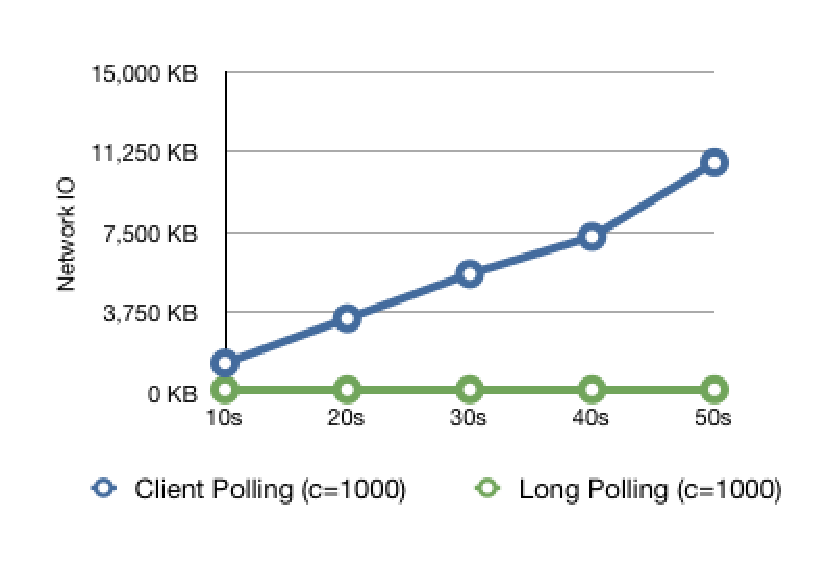
\includegraphics[scale=0.70]{figures/io.eps}
    \caption{Network Traffic of Pull \& Push Models}
    \label{fig:traffic}
\end{figure}


\begin{table}
\centering \caption{\label{tb:mpt_all} Mean Publish Trip Time (second)}
\begin{tabular}{|l|l|l|l|l|l|}
    \hline cc=10 & 10 sec & 20 sec & 30 sec & 40 sec & 50 sec \\
    \hline CP & 0.6 & 0.7 & 0.5 & 0.7 & 0.8 \\
    \hline MLP & 0.1 & 0.0 & 0.1 & 0.2 & 0.1 \\
    \hline ELP & 0.2 & 0.1 & 0.1 & 0.4 & 0.2 \\
    \hline
    \hline cc=100 & 10 sec & 20 sec & 30 sec & 40 sec & 50 sec \\
    \hline CP & 0.8 & 1.1 & 2.5 & 3.1 & 2.7 \\
    \hline MLP & 0.5 & 0.4 & 0.5 & 0.8 & 1.1 \\
    \hline ELP & 0.7 & 0.4 & 0.8 & 1.2 & 0.9 \\
    \hline
    \hline cc=1000& 10 sec & 20 sec & 30 sec & 40 sec & 50 sec \\
    \hline CP & 2.8 & 3.4 & 4.5 & 5.3 & 7.2 \\
    \hline MLP & 2.3 & 2.9 & 2.7 & 3.5 & 3.4 \\
    \hline ELP & 2.4 & 2.8 & 1.8 & 2.4 & 2.9 \\
    \hline
\end{tabular}
\end{table}

\begin{figure}[htb!]
\centering%
    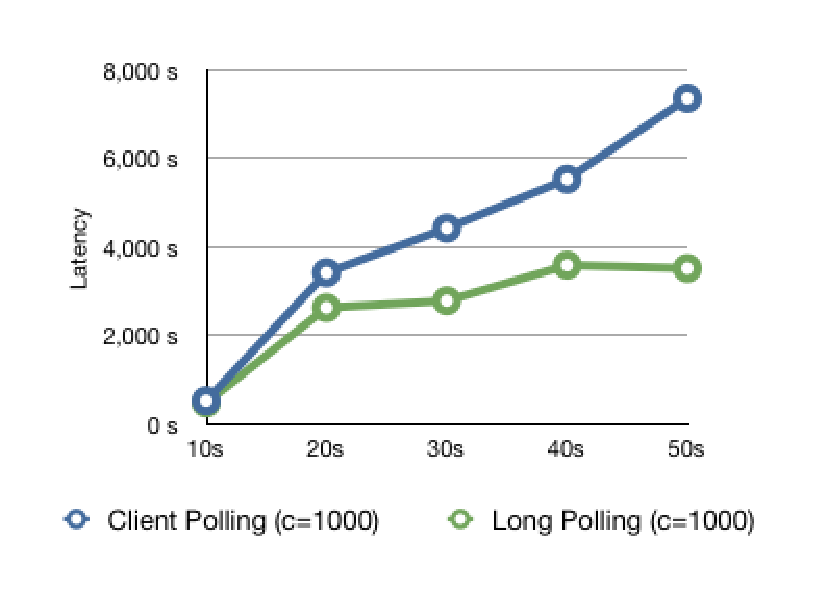
\includegraphics[scale=0.70]{figures/latency.eps}
    \caption{Mean Publish Trip Time of Pull \& Push Models}
    \label{fig:traffic_latency}
\end{figure}

\subsection{Event vs. Thread\\}

Here we compared the performance between event-driven long polling method
and the multithreading long polling method. In the following evaluation
we tested the {\bf server memory usage(SMU)}, {\bf mean publish trip time
(MPT)}, {\bf received message percentage(RMP)} with large number of
active connections(from 500-16000).

Figure \ref{fig:et_memory} shows the server memory usage of both methods.
The event-driven method demonstrates an excellent memory usage as the
number of active connections increases, while the memory usage of 
multithreading method soars rapidly and reaches $100\%$ when the active
connections' number goes to $8000$.

Figure \ref{fig:et_latency} and figure \ref{fig:et_rate}, show the mean
publish trip time and received message percentage. Event-driven method 
significantly excels multithreading method in both evaluation.

Thus we claimed one-polling-request-per-thread approach is not a good 
choice for handling large amount of concurrent connections, as its
memory usage and possible context switch may incur very large overhead.
The event-driven method, on the other hand, demonstrates a better 
performance in memory usage and hosting large concurrency.  

\begin{figure}[htb!]
\centering%
    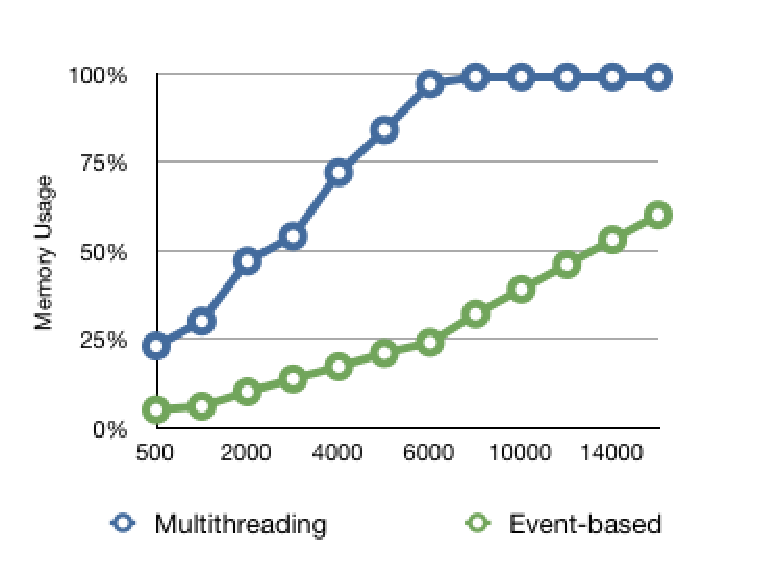
\includegraphics[scale=0.70]{figures/et_memory.eps}
    \caption{Server Memory Usage}
    \label{fig:et_memory}
\end{figure}

\begin{figure}[htb!]
\centering%
    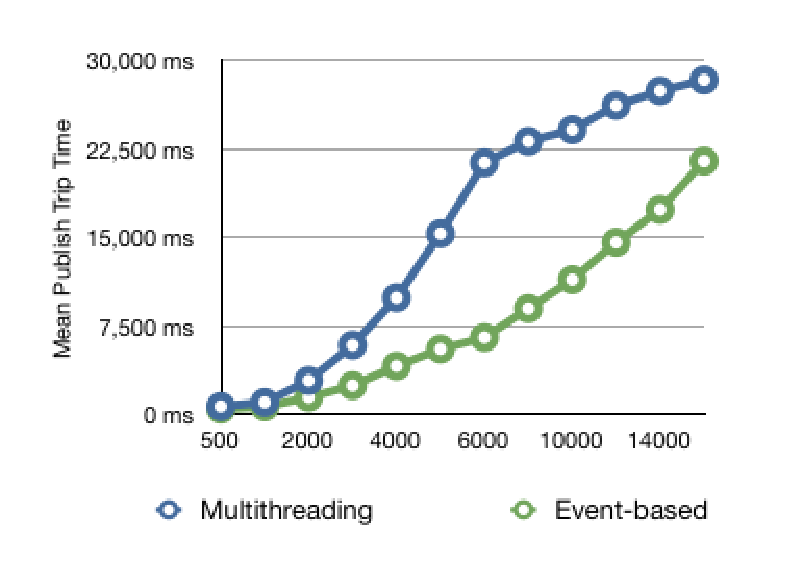
\includegraphics[scale=0.70]{figures/et_latency.eps}
    \caption{Mean Publish Trip Time}
    \label{fig:et_latency}
\end{figure}

\begin{figure}[htb!]
\centering%
    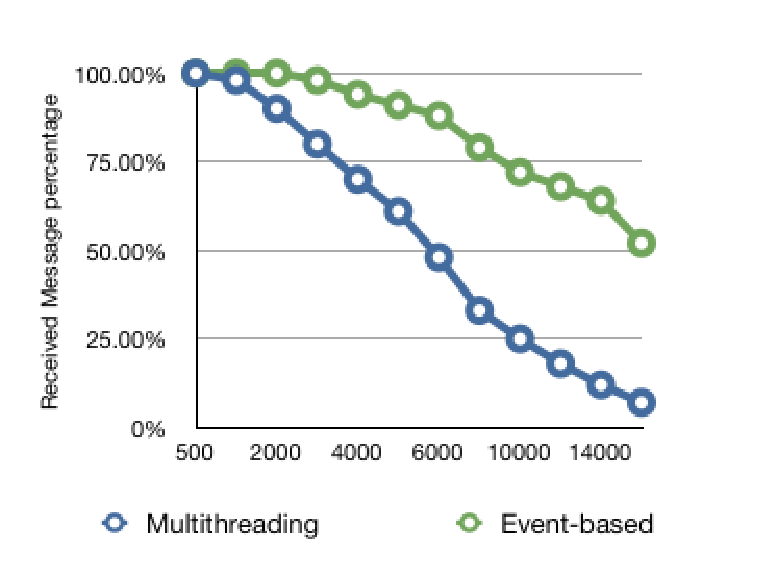
\includegraphics[scale=0.70]{figures/et_rate.eps}
    \caption{Received Message Percentage}
    \label{fig:et_rate}
\end{figure}


\subsection{Extending PushUp Server\\}

\begin{figure}[htb!]
\centering%
    \includegraphics[scale=0.30]{figures/multinode_latency.eps}
    \caption{Mean Publish Trip Time}
    \label{fig:mt_latency}
\end{figure}

\begin{figure}[htb!]
\centering%
    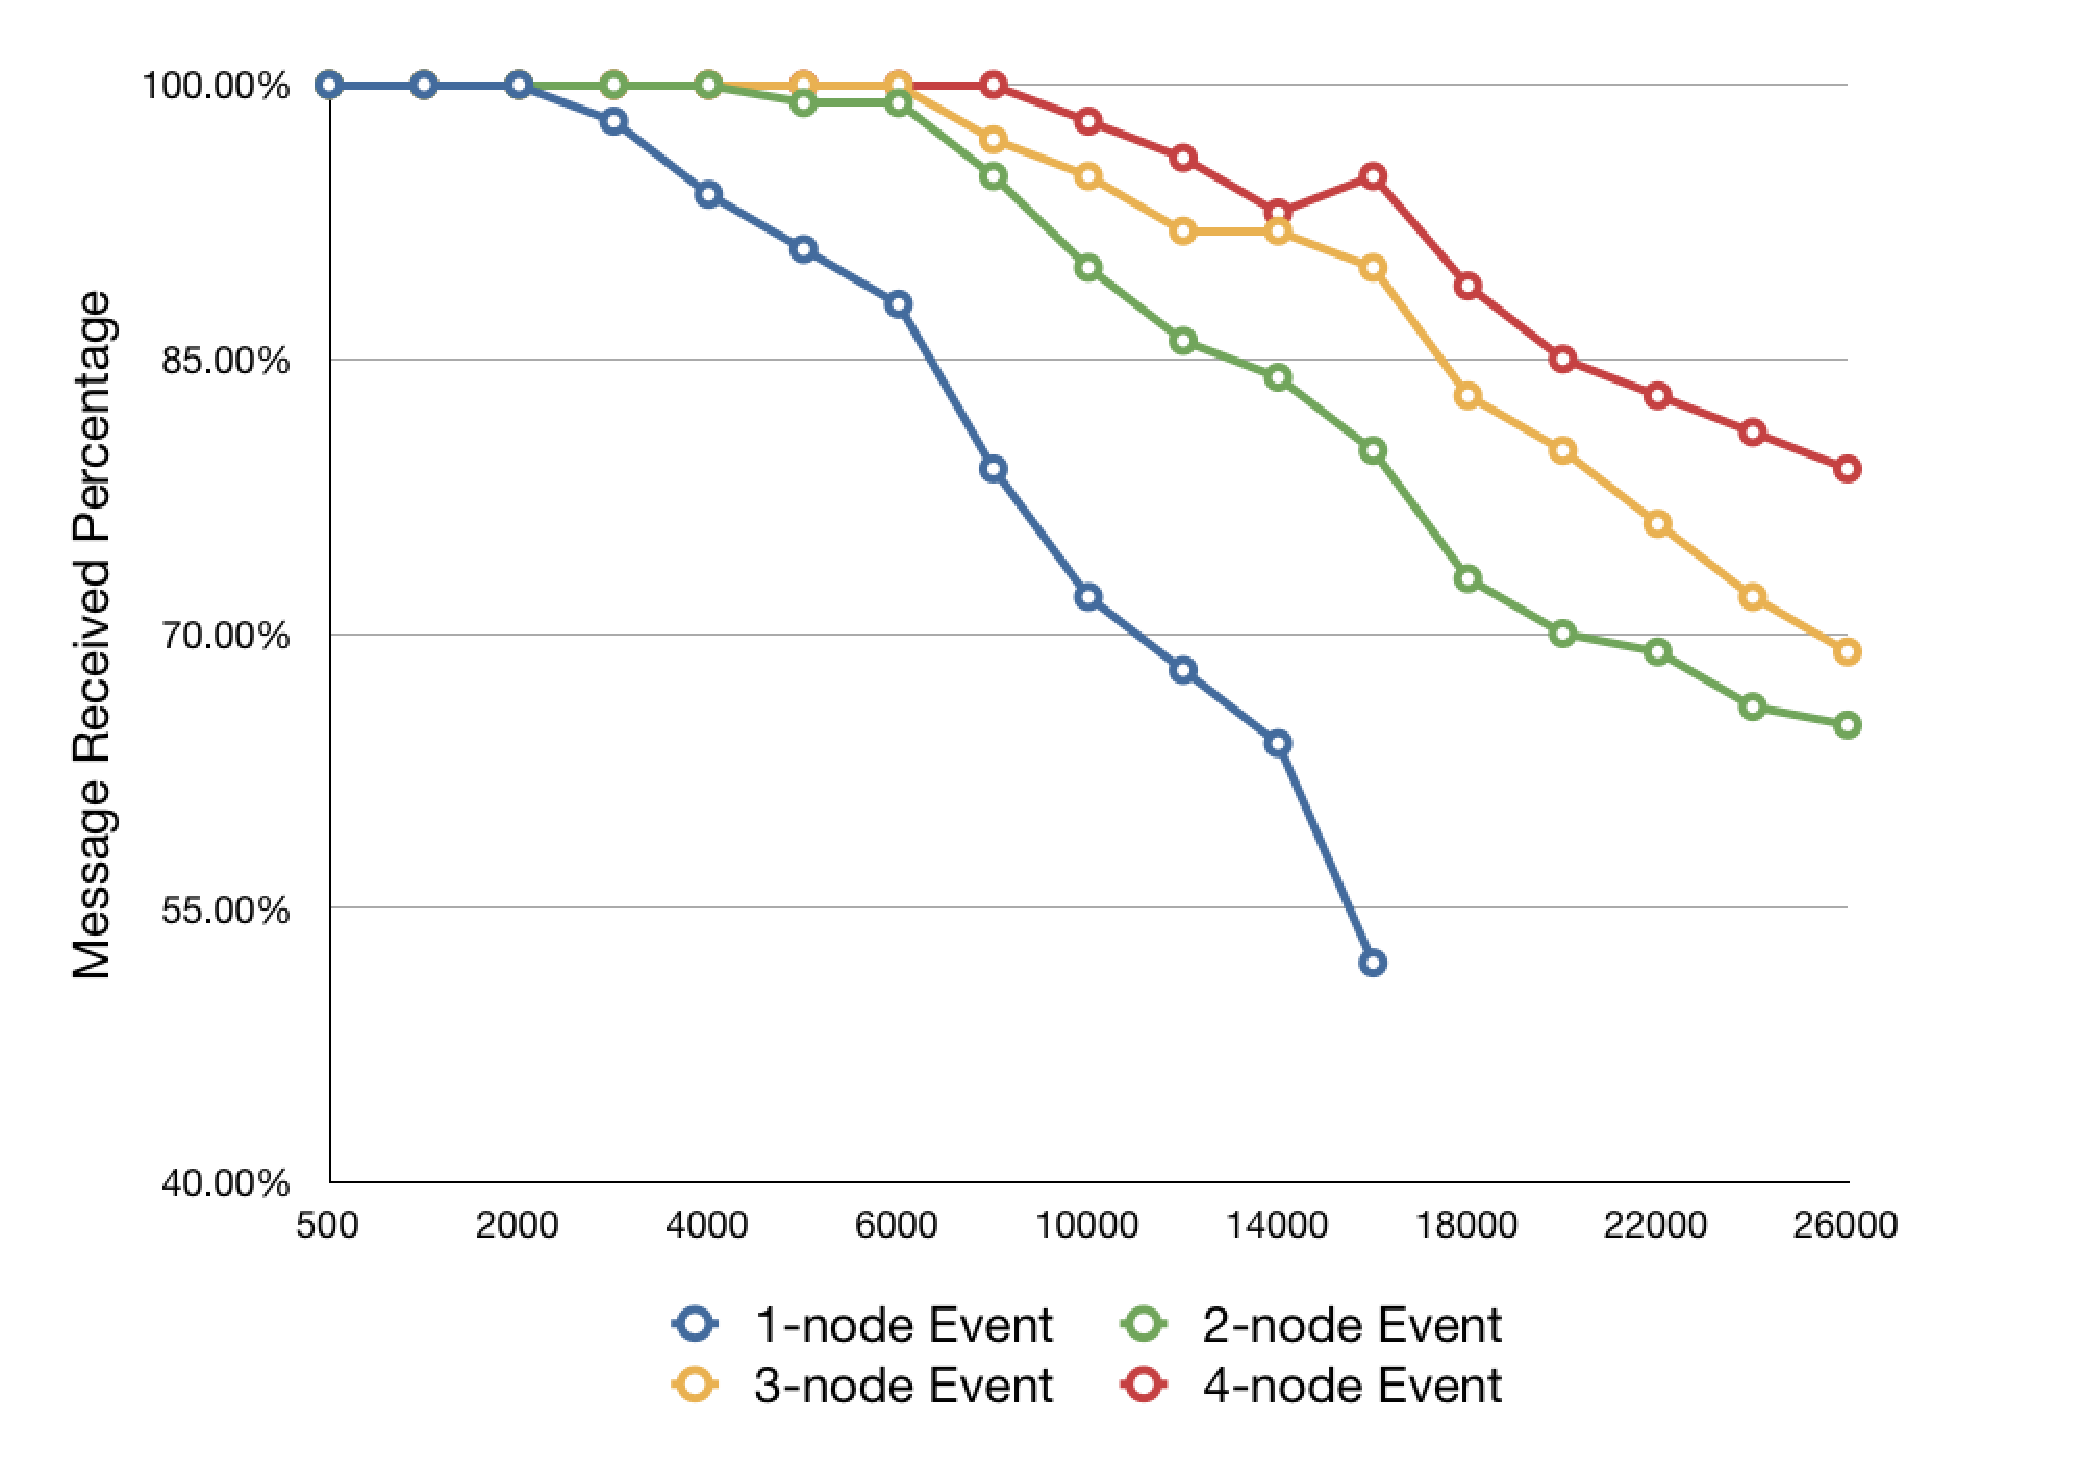
\includegraphics[scale=0.30]{figures/multinode_rate.eps}
    \caption{Received Message Percentage}
    \label{fig:mt_rate}
\end{figure}

As we saw the advantages of PushUp over other event notificaition methods, 
now we would like to extend one PushUp server to $2$,  $3$ and $4$ servers
and see the performance changes as PushUp scales.

In this evaluation, the incoming polling requests will be (almost) evenly 
distributed to each PushUp server. A simple round-robin will be sufficient 
for this task. We used the HAProxy\cite{HAProxy} as a load balancer, which
simply balances the load in the TCP layer.

Figure \ref{fig:mt_latency} and figure \ref{fig:mt_rate}, respectively, show
the {\bf mean publish trip time} and {\bf received message rate} of the 
PushUp servers with different nodes.

These figures verify that the PushUp servers scale almost linearly as the 
number of nodes increases, with a very small overhead in load balancing 
and updates propagation among PushUp servers.


\section{Related Work\\}

\subsection{Event vs. Thread\\}

Some stuff mentioned in the class.

\subsection{Server Push technologies\\}

Full evaluation of the Server Push Technologies: http://academic.research.microsoft.com/Publication/2858750/comparative-evaluation-of-server-push-and-client-pull-architectures-for-multimedia-servers

Some quantitative analysis of many different push technologies:http://www.simonduquennoy.net/papers/duquennoy09consistency.pdf



%
% The following two commands are all you need in the
% initial runs of your .tex file to
% produce the bibliography for the citations in your paper.
\bibliographystyle{abbrv}
\bibliography{sigproc}  % sigproc.bib is the name of the Bibliography in this case
% You must have a proper ".bib" file
%  and remember to run:
% latex bibtex latex latex
% to resolve all references
%
% ACM needs 'a single self-contained file'!
%
%APPENDICES are optional
%\balancecolumns
% That's all folks!
\end{document}
